\documentclass[11pt]{article}

% --- geometry / fonts ---
\usepackage[letterpaper,margin=1in]{geometry}
\usepackage{microtype}
\usepackage[T1]{fontenc}
\usepackage{lmodern}

% --- math / symbols ---
\usepackage{amsmath}
\usepackage{amssymb}

% --- tables ---
\usepackage{booktabs}
\usepackage{array}

% --- figures ---
\usepackage{graphicx}
\usepackage{float}
\graphicspath{{../}{../results/figures/}}

% --- color / links ---
\usepackage{xcolor}
\usepackage[colorlinks=true,linkcolor=blue!55!black,citecolor=blue!55!black,%
            urlcolor=blue!55!black,breaklinks=true]{hyperref}
\usepackage{url}

% --- bibliography (author-year) ---
\usepackage[round,authoryear]{natbib}
\bibliographystyle{plainnat}

% gently absorb the occasional long unbreakable token (code/URLs) instead of
% overflowing into the margin
\setlength{\emergencystretch}{3em}

% allow generous page breaking around floats
\renewcommand{\topfraction}{0.92}
\renewcommand{\bottomfraction}{0.85}
\renewcommand{\textfraction}{0.08}
\renewcommand{\floatpagefraction}{0.80}

\title{Hold Your Fire: Disruption-Aware Failure Monitoring for Coding Agents}

\author{Faizan Ahmed\\
\texttt{faizan@theheadstarter.com}}

\date{\today}

\begin{document}
\maketitle

\begin{abstract}
Coding agents fail mid-trajectory by looping on a broken command, churning edits whose tests never improve, or drifting from the bug. A monitor that predicts failure from a partial trajectory could intervene early, but intervention is double-edged: interrupting a run that would have succeeded causes the very failure it was meant to prevent, a tension we call the Intervention Paradox. Studying local, CPU-only monitors for SWE-agent trajectories, we reach one thesis: accurate prediction is not the goal; calibrated abstention is. On 127k leakage-controlled prefix examples, a 1.14 MB monitor predicts terminal failure at ROC AUC 0.722 with a roughly 13-step lead, bounded by an irreducible early floor we characterize rather than chase. Recast as a selective predictor that abstains on prefixes it cannot yet judge, it cuts false alarms on successful runs by 35\%, and on a live agent it cuts disruptive interventions from 79\% to 7\%, at a fraction of the cost of the local and frontier LLM judges it out-predicts. A paired held-out bootstrap caught validation overfitting five times, so we trust our negative results as much as the positive ones, including that cross-scaffold collapse is a recoverable feature-scale artifact and that monitorability tracks the agent's action space, not its capability. A white-box follow-up on a 30B model and real, contamination-free tasks sharpens the thesis: a penalty targeted at the repeated command breaks 100\% of audited loops, yet on a capable model every eager intervention fails, with no steerable recovery direction, a ``reconsider'' nudge that lowers the solve rate, and gains that come from selection rather than steering. From the intervention side as from the monitoring side, the value lies in restraint.

\end{abstract}
\section{Introduction}
LLM coding agents (SWE-agent, mini-SWE-agent, OpenHands, and similar) operate autonomously over long tool-use trajectories: reading files, editing code, running tests. Many of those trajectories end in failure, and they often telegraph it long before the end: an agent re-runs an identical failing command, or edits the same five lines again and again while the test output never changes. A \emph{monitor} that reads the trajectory prefix and flags impending failure could trigger a cheap corrective intervention (a hint, a reset, a human ping) and save wasted compute.

The catch is the \textbf{Intervention Paradox}: a monitor that fires on a run which was actually going to succeed \emph{disrupts} it. For a disruption-aware monitor the operative cost is therefore not classification error but the \textbf{false-alarm rate on successful runs}, traded against coverage of real failures and the lead time of the warning.

This framing changes what ``good'' means, and it drives our central finding. We can predict failure only \emph{moderately} well from a partial trajectory, and, crucially, that ceiling is \textbf{real, not a modeling deficiency}: a prefix taken ten steps into a run that eventually fails is frequently indistinguishable from a healthy prefix, because the run had not yet gone wrong. No amount of model capacity recovers a signal that is not yet present. The right response is not a better classifier but a monitor that \textbf{abstains} on prefixes it cannot yet judge and commits only when the evidence is there.

Where prior agent and reasoning monitors optimize predictive \emph{accuracy} (process reward models, step verifiers, prefix critics; see Related Work), we are (to our knowledge) the first to frame trajectory monitoring as \textbf{disruption-aware selective prediction}, to pair it with a \textbf{leakage-controlled evaluation protocol} that a candidate must survive on a paired, instance-grouped held-out bootstrap, and to characterize \textbf{when} behavioral monitoring works, across model scale, agent action space, and \emph{prediction time} (post-hoc acceptance $\gg$ early warning). Everything runs locally on CPU; the only paid component is the LLM-judge baseline.

\textbf{Contributions.}

\begin{enumerate}
\item A local, CPU-only failure monitor for SWE-agent trajectories with honest, leakage-controlled performance (AUC 0.722, calibrated, $\sim$13-step lead), and a characterization of \emph{why} that number is a ceiling (\S4.1, \S4.6).
\item \textbf{Selective prediction (abstention) as the deployable form} of the monitor: AUC 0.80 @ 50\% coverage, 35\% fewer false alarms on successful runs, with a risk-coverage curve and a deployable step-gate (\S4.3).
\item A \textbf{cross-scaffold generalization study} (second independent source, OpenHands/CodeAct): naive zero-shot collapses to near-chance (0.53), but \textbf{three free, label-free fixes recover it} (unsupervised feature-distribution alignment (0.59, $\approx$ the in-domain ceiling), an ensemble of transferable submodels (0.60), and abstention (0.66)): the collapse is mostly a feature-\emph{scale} artifact, not absent signal; a \emph{post-hoc acceptance} use transfers fully (0.72) (\S4.4).
\item A controlled finding that \textbf{behavioral monitorability is governed by the agent's \emph{action space}, not its capability}: at matched data budget, within a scaffold monitorability \emph{rises} with capability (0.56$\to$0.76), while a structurally different action space (CodeAct) is intrinsically less monitorable regardless, refuting a ``capable agents fail invisibly'' reading (\S4.8, Fig 10).
\item \textbf{Online validation} on a live local agent showing abstention cuts disruptive interventions 79\% $\to$ 7\% on the same runs (\S4.5).
\item A \textbf{human-validated} account of which failures are catchable early (\S4.7), measured deployment cost, and a baseline study showing cheap structured features \textbf{out-predict local \emph{and} frontier LLM judges} (GPT-5.5, Claude Opus 4.8) at $\sim$1/10,000th the cost (\S4.2).
\item The \textbf{evaluation protocol itself} (a paired instance-grouped held-out bootstrap) surfaced as a methodological contribution that repeatedly caught mirages (\S5).
\item A \textbf{mechanistic, low-disruption intervention for the dominant failure mode (loops)}: a white-box study localizes looping to a causally-steerable layer-8 axis, then shows that the deployable fix is a \textbf{monitor-gated, \emph{targeted} penalty on the specific repeated command}: it breaks 100\% of audited real loops at near-zero disruption, where generic repetition penalties and circuit ablation fail. We carry the honest negative too: breaking the loop does not by itself flip outcomes at 1.5B, which sets up the decisive capable-model experiment we then run (\S4.9, \S4.10).
\item A \textbf{demonstration of the Intervention Paradox on a capable model and real hard tasks} (\S4.10): scaling white-box steering to a 30B MoE (on-device) and running an agentic loop over contamination-free LiveCodeBench, we find a capable model has \textbf{no steerable recovery direction} (its failures are competence, not a behavioral pathology), an eager ``reconsider'' nudge measurably \emph{lowers} the solve rate (5/21 $\to$ 2/21), and the only outcome gain comes from \textbf{selection} (execution-grounded sample-and-vote, 0.55 $\to$ 0.88), closing the paper's outcome-flip question from the intervention side: a monitor's value is restraint, not action.
\end{enumerate}
\section*{Related work}
\textbf{Coding agents and benchmarks.} SWE-bench \citep{jimenez2024swebench} established resolved/ unresolved grading on real GitHub issues; SWE-agent \citep{yang2024sweagent} and OpenHands \citep{wang2024openhands} are widely-used scaffolds with very different action spaces (a shell- command interface vs. CodeAct function-calling). We monitor trajectories from both; our second-source study (\S4.4) deliberately spans these two action spaces, and the public Nebius SWE-agent corpus supplies our training trajectories.

\textbf{Monitoring agent/reasoning trajectories (process supervision).} Most prior work scores intermediate steps to \emph{improve} task success: process reward models and step verifiers \citep{lightman2023verify}, outcome vs. process supervision, trajectory critics, and prefix- based failure predictors. These optimize predictive accuracy. We differ in \emph{objective}: we treat monitoring as a \textbf{disruption-aware decision} in which the dominant cost is a false alarm on a \emph{healthy} run (the Intervention Paradox), and show the deployable form is selective prediction, not a higher-AUC classifier.

\textbf{Selective prediction and the reject option.} Classification with a reject option \citep{chow1970reject}, selective classification and risk-coverage analysis \citep{elyaniv2010foundations,geifman2017selectivenet}, and learning-to-defer \citep{madras2018predict,mozannar2020consistent}. We bring this lens to agent monitoring (the first time to our knowledge), with a deployable \emph{prefix-visible} abstention gate and a risk-coverage curve rather than a single operating point.

\textbf{Confidence calibration.} Temperature scaling and reliability diagrams \citep{guo2017calibration}; isotonic / Platt calibration \citep{zadrozny2002transforming}. Calibration is central both to our gate and to our cross-distribution finding: the monitor's \emph{ranking} transfers while its \emph{probabilities} are target-specific and cheaply recalibrated.

\textbf{Distribution shift and domain adaptation.} Covariate-shift importance weighting \citep{shimodaira2000improving} and correlation alignment (CORAL) \citep{sun2016return}. Our cross-scaffold study uses unsupervised feature-distribution (quantile) alignment, shows the naive transfer collapse is largely a feature-\emph{scale} artifact, and reports which DA techniques do and do not help on this task.

\textbf{LLM-as-a-judge.} Using strong LLMs to evaluate outputs \citep{zheng2023judging}. We include local (qwen2.5-coder) and frontier (GPT-5.5, Claude Opus 4.8) judges as baselines; a 1 MB structured classifier \emph{significantly out-predicts all of them} here at $\sim$10$^4$$\times$ lower cost: a caution for LLM-judge-based monitoring.

\textbf{Positioning / what is new.} Closest to us are prefix-based agent failure predictors; we depart by (i) reframing the task as \textbf{disruption-aware selective prediction}, (ii) foregrounding a \textbf{leakage-controlled paired-bootstrap protocol} that repeatedly caught validation-overfitting, and (iii) characterizing \textbf{when} behavioral monitoring works, across model scale (it \emph{helps}), action-space/scaffold (the dominant factor, recoverable by free alignment), and prediction time (post-hoc acceptance $\gg$ early warning).

\section{Problem setup and data}
\textbf{Trajectories.} We use the public Nebius \texttt{SWE-agent-trajectories} corpus: 80,036 trajectories over 3,591 GitHub issue instances, generated by three model families (swe-agent-llama 70b / 8b / 405b). Each trajectory is a sequence of (thought, action, observation) steps with a terminal success/failure label.

\textbf{Prefixes and labels.} From each trajectory we emit \emph{prefix} examples at increasing step counts; a prefix's label is the trajectory's \textbf{terminal outcome}. This is the honest but deliberately noisy setup: an early prefix of an eventually-failed run is labeled ``fail'' even though nothing has gone wrong yet. We treat that label noise as a first-class object of study rather than hiding it; it is the source of the early floor. The corpus yields \textbf{127,092 prefix examples}.

\textbf{Splitting and leakage control.} All splits are \textbf{grouped by \texttt{instance\_id}} (a repo issue), never by prefix row, so prefixes of the same trajectory (and the same underlying task) never straddle train/test. Split sizes: 81,070 / 20,856 / 25,166 prefix rows over 2,297 / 575 / 719 instances (train / val / test); failure base rate $\approx$ 0.57. We never expose post-hoc fields (the gold patch, eval logs, exit status, future observations). A \textbf{shuffled-label control} gives AUC 0.522, confirming the signal is not leakage. Thresholds and any model selection are done on validation; test is scored \textbf{once}.

\section{Method}
\textbf{Features.} Cheap, structured, prefix-visible signals only, in families: length/pace, action-type counts, file behavior (read-before-edit, edited-never-read), testing behavior, and loop/repetition signals (max command repeat, repeated-exact-command, same-action streaks). Feature extraction scans a bounded recent window, so per-prefix cost is independent of trajectory length. No future information enters a prefix's features.

\textbf{Models.} Logistic regression, random forest, and histogram gradient boosting (HistGradientBoosting), with majority / step-count-only / hand-rule baselines. Probabilities are \textbf{isotonically calibrated} on validation (we report ECE and Brier). HistGradientBoosting is the deployed model.

\textbf{The abstention gate.} A prefix is \emph{committed} (the monitor is allowed to fire) only when \texttt{prefix\_step >= S} \textbf{and} \texttt{|calibrated\_risk - 0.5| >= C}; otherwise the monitor returns ``insufficient evidence'' and stays silent. We sweep \texttt{(S, C)} to produce a \textbf{risk-coverage curve} (AUC on committed prefixes vs. fraction committed), compared against a \emph{random-abstention} control that holds coverage fixed but drops prefixes at random. The gate is wired into the live monitor as an explicit abstain verdict.

\textbf{Evaluation protocol (the rigor).} For every candidate improvement we compute a \textbf{paired instance-bootstrap of the metric delta} on the held-out test set: resample \emph{instances} (not rows), recompute the metric for baseline and candidate on the same resample, and report the delta distribution, its 95\% CI, and the fraction of resamples in which the candidate wins. A change counts only if it survives this on test, not if it merely looked better on validation. \S5 shows why this matters.

\section{Results}
\subsection{Failure is predictable, but only moderately, and that is a real ceiling}
Lightweight monitors predict eventual failure well above chance and above length-only baselines (\texttt{table1\_offline.csv}):

\begin{center}\small
\resizebox{\ifdim\width>\linewidth\linewidth\else\width\fi}{!}{%
\begin{tabular}{llll}
\toprule
model & ROC AUC [95\% CI] & AUPRC & ECE \\
\midrule
majority & 0.500 & 0.569 & 0.007 \\
step-count only & 0.623 [0.607, 0.636] & 0.707 & 0.014 \\
heuristic rules & 0.574 [0.538, 0.607] & 0.632 & 0.012 \\
logistic regression & 0.693 [0.673, 0.711] & 0.762 & 0.018 \\
random forest & 0.719 [0.699, 0.740] & 0.793 & 0.015 \\
\textbf{hist gradient boosting} & \textbf{0.722 [0.700, 0.743]} & 0.792 & \textbf{0.011} \\
\bottomrule
\end{tabular}}
\end{center}
Calibrated risk \textbf{rises over trajectory time for failed runs} ($\approx$0.52 $\to$ 0.78) while staying flat ($\sim$0.5) for successful runs (Figure 1), and the median warning \textbf{lead time is 13 steps} at the deploy threshold (Figure 3); precision-recall against the baselines is in Figure 2, and the monitor is well-calibrated (ECE 0.011; reliability diagram, Figure 11). The shuffled-label control (0.522) rules out leakage.

This 0.722 is honest, not disappointing: terminal-on-prefix labels make some eventually-failed prefixes \emph{genuinely healthy}, an \textbf{irreducible early floor}. \S4.6 shows we tried hard to beat it and could not, which is the motivation for abstention.

\subsection{Cheap structured features beat text, and \emph{out-predict} local and frontier LLM judges}
\begin{itemize}
\item \textbf{Structured $\gg$ step-count-only} (0.722 vs 0.623): the monitor is not merely learning ``long runs fail.'' The dominant risk-raising features are repetition/looping signals and a high search-to-edit ratio (Figure 5), i.e. \emph{visible flailing}, consistent with \S4.7.
\item \textbf{Structured $\ge$ text:} adding TF-IDF text features \emph{lowers} AUC (0.722 $\to$ 0.672).
\end{itemize}
\textbf{The cheap classifier out-predicts every LLM judge we tried}: a local 7B \emph{and} two frontier models, swept across reasoning effort. We give each model the \emph{same} prompt, schema, and prefix renderer (only the model/provider changes) and score it on the same 200 matched test prefixes (\texttt{gpt\_judge*.json}; the classifier is the small-corpus model on this subset, AUC 0.77):

\begin{center}\small
\resizebox{\ifdim\width>\linewidth\linewidth\else\width\fi}{!}{%
\begin{tabular}{lllll}
\toprule
judge (same 200 prefixes) & ROC AUC & wants to intervene & latency/prefix & cost / 200 \\
\midrule
\textbf{structured classifier (1 MB, CPU)} & \textbf{0.768} & N/A & $\sim$9 ms & \$0 \\
qwen2.5-coder:7b (local) & 0.559 & 97\% & 11.6 s & \$0 \\
GPT-5.5: effort low / high & 0.626 / 0.619 & 62\% / 58\% & 2.6 / $\sim$9 s & \$0.44 / \$0.99 \\
Claude Opus 4.8: thinking none / low / high & 0.618 / 0.639 / 0.633 & 46\% / 43\% / 41\% & $\sim$6-8 s & \$2.10-2.70 \\
\bottomrule
\end{tabular}}
\end{center}
Paired instance-bootstraps put the classifier \textbf{significantly ahead of every config} ($\Delta$ +0.13 to +0.21; all CIs exclude 0; $\ge$99\% of resamples favor the classifier). \textbf{Two frontier models from two providers converge at $\sim$0.62-0.64}, so this is not a one-model quirk, and \emph{sweeping the reasoning axis barely moves them}: GPT-5.5 at high effort (0.619) is statistically identical to low (0.626; $\Delta$ $-$0.006, n.s.), and Opus 4.8 extended thinking yields only a small, borderline bump (0.618 $\to$ 0.639; low$-$none $\Delta$ +0.021, 95\% CI [$-$0.001, +0.046], n.s.; low $\approx$ high). The judges are also far too intervention-happy (41-97\%) for a disruption-aware monitor. So cheap structured features don't merely \emph{match} a local judge; they \textbf{significantly out-predict frontier LLMs at $\sim$1/10,000th the cost}; more capability and more thinking buy little-to-no accuracy at this task.

\begin{itemize}
\item \textbf{Measured cost: latency and memory} (\texttt{cost.json}, M4 CPU, psutil RSS). The model is \textbf{1.14 MB on disk} and serves from a \textbf{$\sim$210 MB resident process} (Python + sklearn + model). On the \emph{real} \texttt{Monitor.assess()} path it scores a live prefix in \textbf{$\sim$8.6 ms} (median; p90 $\sim$15-23 ms), dominated by sklearn's per-\texttt{predict} overhead, not compute (feature extraction is 0.14 ms); batched, it does $\sim$390k prefixes/s and scores the \textbf{entire 25,166-prefix test set in <0.1 s}. The LLM judge needs \textbf{4.7 GB} of weights and \textbf{11.6 s/prefix}; so the monitor is \textbf{$\sim$20$\times$ lighter in memory and $\sim$1,300$\times$ faster per prefix} ($\ge$10$^4$$\times$ batched). ``Local, lightweight, CPU-only'' is a measurement, not an adjective.
\end{itemize}
\subsection{The deployable headline: abstention}
The terminal-on-prefix label is noisy early (AUC $\sim$0.63 on early prefixes) and informative late ($\sim$0.81), but ``late'' requires the unknown total length, so it is not directly deployable. The deployable fix is to \textbf{abstain} using only prefix-visible quantities (\texttt{abstention.json}, Figure 6):

\begin{itemize}
\item \textbf{AUC 0.80 at 50\% coverage, 0.83 at 30\%}, vs 0.72 unconditional. A \emph{random}-abstention control stays flat at 0.72: the lift is real selection, not a mechanical artifact of dropping examples.
\item Abstaining on early/uncertain prefixes cuts the \textbf{false-alarm rate on successful runs from 0.090 to 0.059 ($-$35\%)} and improves Brier 0.208 $\to$ 0.167; that is, it directly reduces \emph{disruption} (the metric that matters here) at a modest cost in failure coverage (0.44 $\to$ 0.39) and lead time (13 $\to$ 11 steps).
\item Retraining a separate model \emph{on} the committed regime does \textbf{not} help (0.7915 vs 0.7933; paired delta $-$0.0018, 95\% CI [$-$0.008, +0.005], not significant): the single full model plus a gate suffices.
\end{itemize}
The honest, deployable headline is therefore \textbf{``AUC 0.80 @ 50\% coverage / 0.83 @ 30\% (vs 0.72 unconditional), 35\% fewer false alarms on successful runs''}: higher \emph{and} more useful than the unconditional 0.722.

\subsection{Generalization: full transfer across scale/shell agents; cross-scaffold needs a free alignment step}
Does the monitor work beyond its training distribution? We test three increasingly distant shifts (\texttt{generalization.json}, Figure 7). The answer: \textbf{full transfer when the action space is similar, and partial (recoverable for free) across a structurally different scaffold} (where a naive collapse turns out to be mostly a feature-scale artifact).

\begin{itemize}
\item \textbf{Cross-model (same scaffold).} Train on swe-agent-llama-70b \emph{excluding} the test tasks, test on 8b + 405b (unseen models \emph{and} tasks): AUC \textbf{0.735 $\to$ 0.697} (gap +0.037). Calibration degrades (ECE 0.00 $\to$ 0.060) but \textbf{recalibration restores 0.021}.
\item \textbf{Cross-family, shell-style scaffold.} Apply the offline monitor to \emph{live} qwen2.5-coder traces from mini-SWE-agent (a different agent, but still a \emph{shell-command} action space): AUC \textbf{0.674}, above chance; risk \emph{levels} inflate (over-firing), which abstention/recalibration counteract.
\item \textbf{Second independent source, \emph{structurally different} scaffold (OpenHands/CodeAct): a collapse that is mostly a \emph{fixable scale artifact}.} We score the frozen monitor zero-shot on \textbf{500 OpenHands (CodeAct) trajectories} over 500 SWE-bench-Verified instances (\texttt{togethercomputer/CoderForge...}, parsed through the \emph{same} feature pipeline). Naively, AUC \textbf{collapses to 0.525} (near chance) with severe over-firing (success-prefix risk 0.72 vs 0.45). But the failure \emph{structure} is shared: the most predictive features point the same direction as on Nebius (more searching/reading/repetition $\to$ fail); only their \textbf{scale} differs (OpenHands reads 11.8 vs 2.4 per prefix), so the frozen tree's splits misfire. \textbf{Three free, label-free fixes recover most of the signal:}
\item \textbf{Unsupervised feature alignment} (quantile-map each target feature onto the source marginal) lifts zero-shot AUC \textbf{0.525 $\to$ 0.591}, essentially matching the \textbf{in-domain ceiling of 0.603} (5-fold CV, a model trained \emph{on} OpenHands), i.e. alignment recovers nearly all achievable signal with \textbf{zero target labels}.
\item \textbf{An ensemble of transferable feature-family submodels}, tree-on-volume (mapped) $\oplus$ \emph{scale-invariant} repetition (the loop submodel applied \textbf{raw}, no mapping needed) $\oplus$ a linear model (mapped, smoother cross-domain extrapolation), rank-averaged, reaches \textbf{0.604}, slightly \emph{exceeding} the in-domain single model because the source submodels train on 100k+ examples and decorrelate (pre-specified composition, not tuned on target).
\item \textbf{Abstention} (the \S4.3 gate; deployable absolute step-floor) lifts the ensemble to \textbf{0.66 at $\sim$44\% coverage}.
\end{itemize}
If a \emph{few} target labels are available (the few-shot setting), rank-averaging the transferred ensemble with a small in-domain model, which makes \emph{different} errors, adds a further step: \textbf{0.62 full coverage / 0.68 with abstention}.

\textbf{The biggest lever, though, is reframing \emph{when} you predict.} The per-prefix AUC averages over noisy \emph{early} prefixes (an exploring agent looks identical whether it will resolve or not). At the agent's \textbf{final prefix} (a natural, fully-deployable post-hoc patch-acceptance gate: predict when the agent finishes, to accept / retry / escalate), the early-prefix noise is gone and AUC jumps to \textbf{0.722 zero-shot / 0.728 few-shot}, i.e. \emph{Nebius parity (0.722)}, cross-scaffold, free. So cross-scaffold \emph{early-warning} is genuinely hard on the CodeAct scaffold (0.60-0.66), but \emph{post-hoc acceptance} is not (0.72): the information is there at the trajectory level; only the early prefixes lack it. ($\sim$16 further domain-adaptation, ensemble, and selective-prediction techniques were tested and did \emph{not} beat this frontier, enumerated in the supplement: evidence the $\sim$0.60 per-prefix early-warning ceiling is an information limit, not a missing technique.)

So the ranking \emph{does} partially transfer to a structurally different scaffold once distributions are aligned (the naive collapse was largely a feature-\emph{scale} artifact, not absent signal), and a \textbf{post-hoc acceptance} use (judging at the final step) transfers \emph{fully} (0.72), cross-scaffold and free. \emph{Why} the residual early-warning gap belongs to the scaffold rather than the agent's capability is the controlled finding of \S4.8.

\subsection{Online validation on a live agent}
We integrate the monitor into a local mini-SWE-agent + Ollama loop and, to measure disruption \emph{confound-free}, capture \textbf{25 live runs} (qwen2.5-coder:7b; 14 succeeded, 11 failed) in shadow mode, then \textbf{replay} the gated vs. ungated monitor over the \emph{same} trajectories with the gate fixed from the offline study:

\begin{center}\small
\resizebox{\ifdim\width>\linewidth\linewidth\else\width\fi}{!}{%
\begin{tabular}{lll}
\toprule
metric (on the same 25 runs) & ungated & gated (abstain) \\
\midrule
\textbf{disruption} (successful runs ever fired on) & \textbf{78.6\%} & \textbf{7.1\%} \\
\textbf{coverage} (failed runs caught) & 72.7\% & 45.5\% \\
\bottomrule
\end{tabular}}
\end{center}
Under the cross-agent shift the offline monitor over-fires badly (interrupting $\sim$79\% of \emph{successful} runs); abstention cuts that $\sim$\textbf{10$\times$} to 7\%. The reduction is robust at this N: paired bootstrap over the 14 successful runs gives \textbf{0.71, 95\% CI [0.50, 0.93]}, with 100\% of resamples positive (the coverage cost, 0.27, is real but less precisely estimated). A separate forced-intervention run (a low-disruption ``loop-guard''; Figure 4) changed \textbf{no outcomes} (0 recoveries, 0 disruptions) and trimmed wasted steps (40 $\to$ 31); measuring \emph{outcome flips} on a capable model and real tasks is the subject of \S4.10. \textbf{Deployment lesson:} tune the gate to the target's trajectory-length distribution: a step floor right for long traces over-abstains on short runs.

\subsection{The ceiling is real (supporting)}
We tried to raise 0.722 four ways (advanced/interaction features, a decorrelated ensemble, more failure data, and a sequence model) and got \textbf{$\le$ +0.003} (only the ensemble survived the paired test, at +0.0030, 95\% CI [$-$0.0006, +0.0066]). We then attacked the \emph{label} itself with two ``cleaner-label'' reformulations (weak-supervision relabeling and a survival/hazard model with monotone risk) and both \textbf{failed to lift the early prefixes} (early-prefix AUC unchanged at 0.633). The conclusion is structural: early failure is genuinely undetermined or driven by task difficulty that does not transfer across an instance-grouped split. This is \emph{why} abstention (skip the early prefixes) is the right move, not relabeling.

\subsection{What is catchable early, human-validated (supporting)}
We did not trust the regex failure-mode labeler. One author \textbf{blind-labeled 50 prefixes} (40 confidently-flagged failures + 10 missed failures) by reading the actual actions/observations, then joined to the heuristic (\texttt{human\_validation.json}, Figure 9). The result is a correction \emph{and} a confirmation:

\begin{itemize}
\item The regex calls 88\% of flagged failures ``looping''; blind reading finds only 40\% are \emph{tight} loops (precision 0.37, recall 0.94). Most of the rest is \textbf{patch-churn}: varied edits whose tests never improve (permuting a date string while ignoring the real \texttt{NameError}; hard-coding \texttt{if name=="bla": return []} to pass a case).
\item But the \emph{family-level} story holds: 70\% of confidently-caught failures are \textbf{repetition / no-progress} behavior (loops + churn); coarse agreement with the heuristic is 0.68.
\item The observability contrast survives: 70\% of \emph{missed} failures are genuinely \emph{not-observable} or \emph{insufficient-context}: the subtle prefixes the early floor and abstention concede.
\end{itemize}
So the catchable failures are dominated by \textbf{visible repetition and churn} (which motivates loop/no-progress interventions directly), while missed failures are genuinely subtle, and ``looping'' should be read as the broader ``repetition/no-progress'' family.

\subsection{Monitorability is governed by the \emph{action space}, not the agent's capability}
\S4.4 left a question about the residual cross-scaffold early-warning gap: is it because OpenHands' agent is \emph{more capable} (and fails more subtly), or because of its \emph{action space}? We settle it with a controlled analysis (Figure 10, \texttt{capability\_monitorability.json}). The obvious confound is data size (a small in-domain sample yields low AUC from starvation, not difficulty), so we measure each agent's in-domain monitorability at a \textbf{matched 60-instance budget} (20 random subsamples), and plot it against agent capability (trajectory success rate). Within-Nebius (8b/70b/405b: same shell scaffold, overlapping tasks) is the controlled comparison; OpenHands is a different-scaffold point.

The result is clean and, for us, counter-intuitive:

\begin{itemize}
\item \textbf{Within a scaffold, monitorability \emph{rises} with capability.} swe-agent-llama 8b $\to$ 70b $\to$ 405b: AUC \textbf{0.56 $\to$ 0.62 $\to$ 0.76} as success climbs 0.41 $\to$ 0.66. The \emph{most} capable shell agent is the \emph{most} monitorable: the opposite of ``capable agents fail invisibly.''
\item \textbf{The scaffold is the dominant driver.} OpenHands/CodeAct, capability \emph{between} 70b and 405b, is the \textbf{least} monitorable (0.53), sitting far below the shell trend.
\end{itemize}
So behavioral monitorability is a property of the agent's \textbf{action space}: a shell-command interface yields observable failure (looping, repeated errors), while CodeAct's verbose exploration leaves \emph{early} prefixes uninformative. Capability does not erode it; within a scaffold it helps. This refutes a ``capability ceiling'' reading of \S4.4, reframes \emph{when/where} behavioral monitoring works, and predicts that \textbf{a monitor trained on a target scaffold's traces (or a multi-scaffold mix) is the path to cross-scaffold early warning}, not a better feature or a smaller, weaker agent.

\subsection{A mechanistic, low-disruption intervention for the dominant failure mode (loops)}
The Intervention Paradox makes \emph{low-disruption} interventions disproportionately valuable: the less an intervention perturbs a healthy run, the more freely a monitor can afford to fire it. Loops, an agent re-running an identical failing command, are both the \textbf{most catchable} failure (\S4.7) and the most natural target for a \emph{surgical} fix. We ran a white-box mechanistic-interpretability follow-up on \textbf{Qwen2.5-Coder-1.5B-Instruct} (raw forward hooks; full study, code, and artifacts in \texttt{mech\_interp/}) asking: does the agent \emph{internally represent} ``I am repeating an unproductive command,'' is that representation \textbf{causally} responsible for looping, and can the loop be broken \textbf{without} the disruption of an external reset? The results are mixed, and the paired-bootstrap discipline of \S5 again separates a real effect from a confound.

\begin{itemize}
\item \textbf{The looping signal is real and strong.} In a loop context the model prefers to repeat by \textbf{+0.35 nats} (log-prob repeat $-$ novel action) synthetically, and \textbf{+2.33} on 24 of the monitor's \emph{audited real loops}: verbatim repetition pulls the copy mechanism harder than the synthetic case.
\item \textbf{A naive ``loop'' probe hits AUC 1.000, and it is a length confound}, exactly the mirage the paired-bootstrap protocol exists to catch: length alone separates the classes, and steering that confounded direction does \emph{not} break loops. With token length \emph{exactly} controlled, a layer-8 ``are my tests resolving?'' axis is genuinely present and \textbf{causally} steerable (monotonic dose-response, random/orthogonal controls inert, output coherence preserved).
\item \textbf{But representation- and circuit-level edits do not break the loop on-policy.} Single-direction steering gets \textbf{0\% loop-escape} and disrupts \emph{healthy} runs before it touches loop runs; the re-run behavior is \textbf{distributed} (genuine induction heads, e.g. L19H3 places 0.97 of its decision-token attention on the prior command, but no single ``loop head''), so head ablation is \textbf{0\% escape + 60\% disruption}. Off-the-shelf decoding tricks fail here too: always-on \texttt{repetition\_penalty} and \texttt{no\_repeat\_ngram} get \textbf{0\% escape} on these strong verbatim loops \emph{and} \textbf{0.5-0.9 disruption} of productive repetition.
\item \textbf{What works is targeting.} A \textbf{monitor-gated logit penalty on the \emph{specific} repeated command's tokens}, the command the monitor already identifies, breaks \textbf{100\%} of the real loops into \emph{coherent} alternatives (\texttt{git status}, \texttt{open} a new file) at \textbf{$\sim$zero} disruption off-loop. The contribution is \emph{targeting}, not gating and not a generic repetition penalty.
\end{itemize}
This is now a first-class intervention in the deployed system (\texttt{loop\_break}): when the monitor flags a loop it names the repeated command and emits a targeted action: a forbid-this-command message for message-only backends (e.g. Ollama), and the equivalent token-level logit penalty for white-box backends.

\textbf{The looping representation is family-wide; only the lever is small-model.} Re-running the length-matched battery (loop / varied-fail / progress) on Qwen2.5-Coder at 0.5B, 1.5B, 3B, 7B, and 14B (4-bit, on-device, MLX), the identical-command-repetition signal is linearly decodable at ceiling at every scale: the length-matched loop-vs-varied-fail diff-of-means reaches grouped-CV AUC \textbf{1.00}, and \textbf{$\ge$0.95} after decorrelating from context length (against a 0.90 length-only baseline), across a 28$\times$ size range. Bigger same-family models are not blind to looping; they \emph{represent} the distinction just as cleanly. What is small-model-specific is the \emph{behavior} (only a weak model actually falls into the rut) and the \emph{causal lever} (single-direction steering breaks loops at 1.5B; \S4.10 finds a capable 30B has no steerable recovery direction). Monitorability rests on the representation, which scales; the intervention rests on the behavior, which does not (\texttt{scale\_localize.json}).

\textbf{The honest ceiling, and the follow-up it sets up.} A Tier-2 outcome test (a real sandboxed agent loop on six single-edit, \emph{solvable} bug-fix tasks, control vs. targeted-penalty) shows the intervention \textbf{breaks the loop live every time} yet moves task success \textbf{0/6 $\to$ 0/6}: at 1.5B the agent has a broken mental model (it edits the \emph{test call}, never reads the source), so un-sticking only routes it to a different dead end. \textbf{Un-sticking is necessary but not sufficient; the outcome-flip is capability-gated.} A working loop-breaker alone does not improve outcomes with a weak model, which sets up the decisive follow-up the whole paper has pointed to, a \emph{capable} model on \emph{real} hard tasks, which \S4.10 now runs.

\subsection{The decisive experiment, run: a capable model on real hard tasks}
Does \emph{any} intervention flip outcomes on a \textbf{capable} model and \textbf{real} tasks? We ran this locally two ways: white-box steering scaled to a \textbf{30B mixture-of-experts} (on-device, 4-/3-bit, via MLX), and an agentic loop over \textbf{LiveCodeBench}: contamination-free 2025 competitive-programming problems with hidden tests, where a capable model genuinely struggles (a 7B solves 81\% of easy problems and \textbf{0\%} of medium). Three findings, all point the same way: toward restraint, not intervention.

\begin{itemize}
\item \textbf{Capable models get stuck, but not in a \emph{steerable} way.} The weak model's loop is a genuine behavioral axis: in controlled, length-matched probes, steering drives loop-escape 0\%$\to$100\% on held-out synthetic families at 1.5B, and the recovery direction is decodable on-policy at grouped-CV AUC 0.94 (breaking \emph{real} on-policy loops still needs the targeted penalty of \S4.9, but a behavioral lever demonstrably exists). The capable model has no such lever: across four independent contrasts (constructed stuck-states, on-policy rollouts, investigate-vs-act, and progress-vs-flail) it neither loops nor hesitates, so there is nothing for a direction to push. Its failures are \textbf{competence}, not a behavioral pathology, and competence is not a steerable direction.
\item \textbf{The Intervention Paradox, demonstrated.} Tested \emph{paired} against normal test feedback, a monitor-gated ``stop and reconsider your approach'' nudge, the obvious eager intervention, \emph{lowered} the solve count on the problems where the agent was failing (\textbf{5/21 $\to$ 2/21}): on the recoverable ones the agent was iterating toward its own fix and the nudge disrupted it (4/5 $\to$ 2/5), and on the rest it could not help. This is the first \textbf{demonstrated} outcome effect of an eager intervention on a capable model and real tasks, and it is \emph{negative}, direct evidence for the thesis that a monitor's value is calibrated restraint, not eager action.
\item \textbf{What improves outcomes is \emph{selection}, not steering.} Most capable-model failures on \emph{reachable} problems are an \textbf{elicitation gap}, not a competence wall: the correct solution is already in the distribution (pass@k $\gg$ pass@1). Steering toward a ``correctness'' direction fails (the linear probe is a mirage: AUC 0.75 on teacher-forced codes but 0.45 on fresh samples, and additive steering only disrupts); the model's own self-verification is a weak selector (+0.08 pass@1). The lever that works is execution-grounded \textbf{selection} (sample K, run them on the public examples, emit the consensus), lifting pass@1 from \textbf{0.55 to 0.88}. This improves the \emph{generator}, not the monitor, and reinforces the same boundary: you help a capable agent by selecting among its outputs, not by nudging its process.
\end{itemize}
\textbf{Net.} The decisive experiment is no longer open, and its answer sharpens the thesis. The only behavioral intervention that helped was the \emph{surgical, monitor-identified} loop-break (\S4.9); every \emph{eager} or \emph{steering} intervention on a capable model either did nothing (competence) or backfired (the Intervention Paradox). Caveats remain (local scale: 7B and 3-bit 30B; small per-problem N of 8 to 21 problems on the outcome sub-results; and a still-pending SWE-bench-in-Docker confirmation at larger budget), but the direction is unambiguous: for capable coding agents, monitoring's job is to know when \emph{not} to act, and the outcome wins come from \textbf{selection, not steering or nudging.}

\section{The evaluation protocol as a contribution: ``validation lies''}
Our headline contribution is as much \emph{how} we evaluate as \emph{what} we find. Five separate times, a change that won on validation was \textbf{no better or significantly worse} on the held-out, instance-grouped test set (\texttt{validation\_vs\_test.json}, Figure 8; baseline test AUC 0.7214):

\begin{center}\small
\resizebox{\ifdim\width>\linewidth\linewidth\else\width\fi}{!}{%
\begin{tabular}{lll}
\toprule
change & validation AUC & held-out test AUC \\
\midrule
advanced features & 0.7247 & 0.7244 \\
val-selected feature set & 0.7259 & 0.7211 \\
sequence GRU & 0.7255 & 0.7163 \\
label position-weighting & 0.7288 & 0.7158 \\
survival GRU & 0.7255 & 0.7163 \\
\textbf{ensemble (survives)} & 0.7255 & \textbf{0.7244} \\
\bottomrule
\end{tabular}}
\end{center}
Only the ensemble survived. Most agent-monitoring papers report one number on one split; the gap between that and a real effect is exactly this \textbf{paired instance-bootstrap on a grouped held-out test}, and it is why we trust our \emph{negative} results (the ceiling, the irreducible floor, the failed cleaner-labels) as much as the positive ones. We recommend it as standard practice for trajectory-monitoring work.

\section{Limitations and future work}
We state the boundaries plainly; several need compute or data beyond a local CPU setup.

\begin{itemize}
\item \textbf{Cross-scaffold early-warning needs a free alignment step; the residual gap is the \emph{scaffold}, not capability.} Training is on Nebius SWE-agent (shell-command) trajectories. \S4.4 tests a \emph{second independent source} (500 OpenHands/CodeAct trajectories): naive zero-shot collapses (0.53), recoverable for free to 0.59 (feature alignment), 0.60 (transferable-submodel ensemble), and 0.66 (abstention), all label-free; post-hoc acceptance transfers fully (0.72). A controlled, data-budget-matched analysis (Fig 10) shows the residual \emph{early-warning} gap is driven by the \textbf{CodeAct action space}, not capability: within a scaffold, monitorability \emph{rises} with capability (8b$\to$405b: 0.56$\to$0.76). Whether a multi-scaffold-trained monitor lifts CodeAct early-warning is open, and we rely on a single OpenHands source and one model.
\item \textbf{The outcome-flip, now demonstrated (in the honest direction).} Whether an intervention flips outcomes on a capable model and real tasks, raised in \S4.5 and \S4.9, is settled in \S4.10 (LiveCodeBench, contamination-free hard tasks; white-box steering scaled to a 30B MoE). The demonstrated effect of an \emph{eager} intervention (a ``reconsider'' nudge) is \textbf{negative} (solve count 5/21 $\to$ 2/21, the Intervention Paradox); a capable model has \textbf{no steerable recovery direction} (its failures are competence, not a behavioral pathology); and the only outcome gain comes from \emph{selection}, not intervention (sample-and-vote on the public tests, 0.55 $\to$ 0.88). Residual caveats: local scale (7B, 3-bit 30B), small per-problem N (8-21 problems) on the outcome sub-results, and a full SWE-bench-in-Docker confirmation at larger budget is future work, but it would test \emph{more} of the same direction, not a different one.
\item \textbf{Modest online N.} 25 live runs on one model (qwen2.5-coder:7b) and toy tasks; the disruption reduction is significant but small-N.
\item \textbf{Single annotator} for the human audit: blind to the per-item heuristic label, but not an inter-rater study.
\item \textbf{The LLM-judge baseline (\S4.2) uses paid APIs} (GPT-5.5, Claude Opus 4.8): the only non-local component of the study, and purely a comparison point; the deployed monitor is 100\% local. Minor methodological asymmetry: Opus via OpenRouter returns JSON via \texttt{json\_object} + tolerant parse while GPT-5.5 uses strict \texttt{json\_schema}; both yield 0\% invalid JSON, so this does not bias the AUC. The judge comparison is on a 200-prefix matched subset of the small corpus (classifier 0.77 there vs the 0.722 full-corpus headline).
\end{itemize}
None of these undercut the thesis (accurate prediction is not enough; calibrated abstention is the deployable form); they bound how far the online and cross-source claims reach, and we are explicit about which numbers are illustrative.

\section{Conclusion}
For coding-agent failure monitoring, the goal is not a higher AUC: it is a monitor that knows when it cannot tell. A CPU-only, leakage-controlled monitor that serves from $\sim$210 MB of RAM predicts failure at AUC 0.722 with a 13-step lead, and \emph{significantly out-predicts} both a local 7B judge and two frontier LLM judges (GPT-5.5, Claude Opus 4.8) at $\sim$20$\times$ less memory and $\sim$1,300$\times$ lower latency. Most importantly, \textbf{reframed as a selective predictor that abstains} it reaches AUC 0.80 at 50\% coverage and cuts disruptive interventions on a live agent from 79\% to 7\%. The ranking generalizes across model scale and shell-style agents; cross-scaffold (CodeAct) the naive collapse is mostly a feature-scale artifact that free distribution alignment, a transferable-submodel ensemble, and abstention largely recover (0.53$\to$0.66), and a controlled analysis shows behavioral monitorability is governed by the agent's \textbf{action space, not its capability} (within a scaffold it \emph{rises} with capability). The accuracy ceiling is real and characterized, which is precisely why abstention, not a bigger model, is the right engineering answer. Beyond \emph{when} to fire, we also probe \emph{what} to fire: a white-box study turns the dominant failure mode (loops) into a low-disruption, monitor-gated \textbf{targeted} loop-breaker that breaks 100\% of audited real loops at near-zero disruption. Running the decisive follow-up that the monitoring results point to, a capable model on real, contamination-free hard tasks, we find that it \emph{confirms restraint}: a capable model has no steerable recovery direction, an eager ``reconsider'' nudge measurably backfires (a demonstrated Intervention Paradox: 5/21 $\to$ 2/21), and what lifts outcomes is selection, not steering (sample-and-vote, 0.55 $\to$ 0.88). We release the code, the artifacts, and, as a first-class contribution, the paired held-out evaluation protocol that kept us honest.

\section*{Figures}
*All figures regenerate from saved artifacts via \texttt{python scripts/make\_report.py} (Figs 1-9, 11)
and \texttt{scripts/run\_capability\_monitorability.py} (Fig 10). Paths are relative to the repo root.*
\begin{figure}[t]\centering
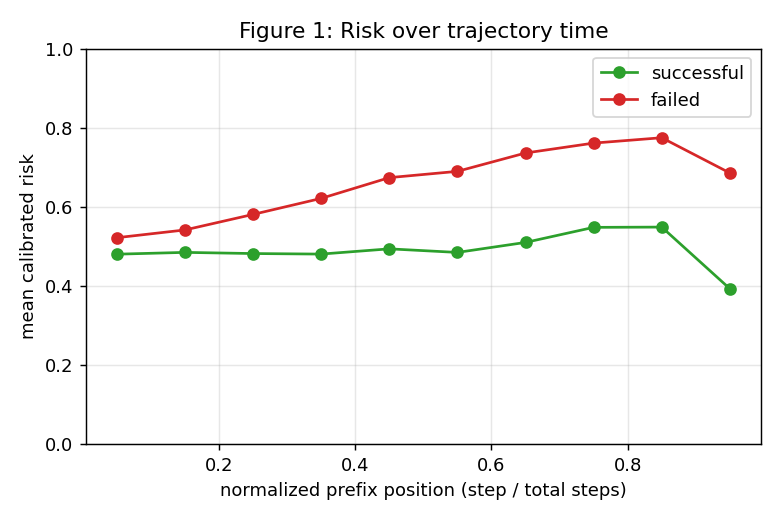
\includegraphics[width=.82\linewidth]{../results/figures/fig1_risk_by_position_offline_full.png}
\caption{\textbf{Risk over trajectory time.} Calibrated failure risk vs. normalized prefix position: it rises for eventually-failed runs ($\approx$0.52$\to$0.78) while staying flat ($\sim$0.5) for successful runs. The signal accumulates over time; early prefixes are near-uninformative (the irreducible floor).}
\end{figure}
\begin{figure}[t]\centering
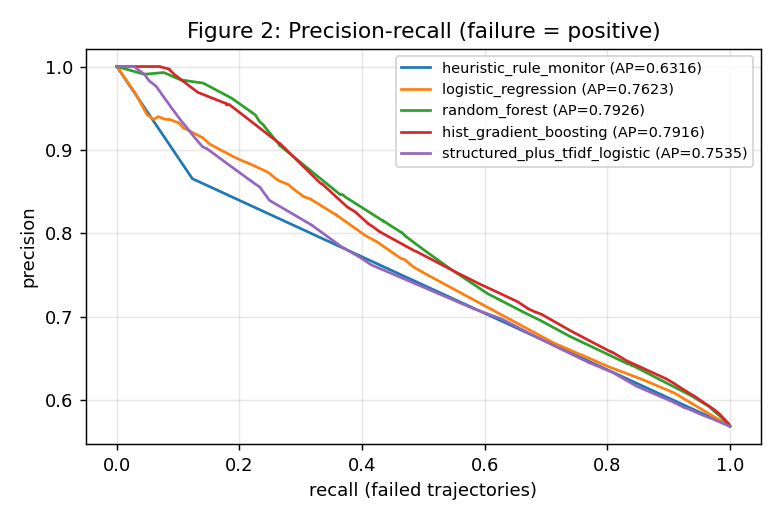
\includegraphics[width=.82\linewidth]{../results/figures/fig2_pr_curves_offline_full.png}
\caption{\textbf{Precision-recall (failure = positive).} The structured monitor vs. length-only and heuristic baselines (with the local LLM-judge overlay). Cheap structured features dominate the length-only and rule baselines.}
\end{figure}
\begin{figure}[t]\centering
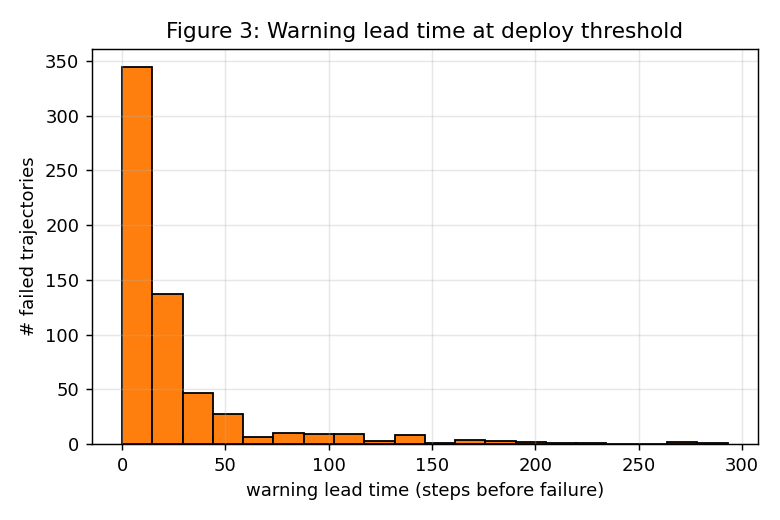
\includegraphics[width=.82\linewidth]{../results/figures/fig3_leadtime_offline_full.png}
\caption{\textbf{Warning lead time.} Distribution of steps between the first alarm and the trajectory end at the deploy threshold; median $\approx$ 13 steps.}
\end{figure}
\begin{figure}[t]\centering
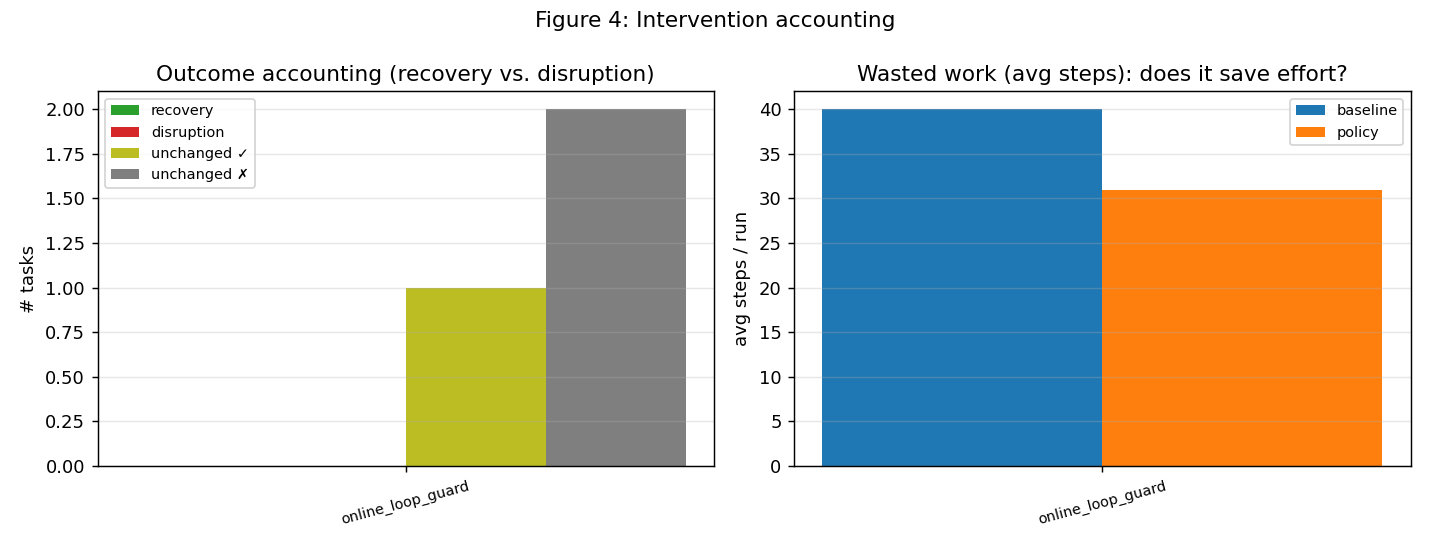
\includegraphics[width=.82\linewidth]{../results/figures/fig4_intervention_accounting.png}
\caption{\textbf{Online intervention accounting.} Loop-guard vs. baseline: outcome changes (0 recoveries / 0 disruptions) and average steps (40$\to$31). The low-disruption gate breaks nothing while trimming wasted work (small-N, illustrative).}
\end{figure}
\begin{figure}[t]\centering
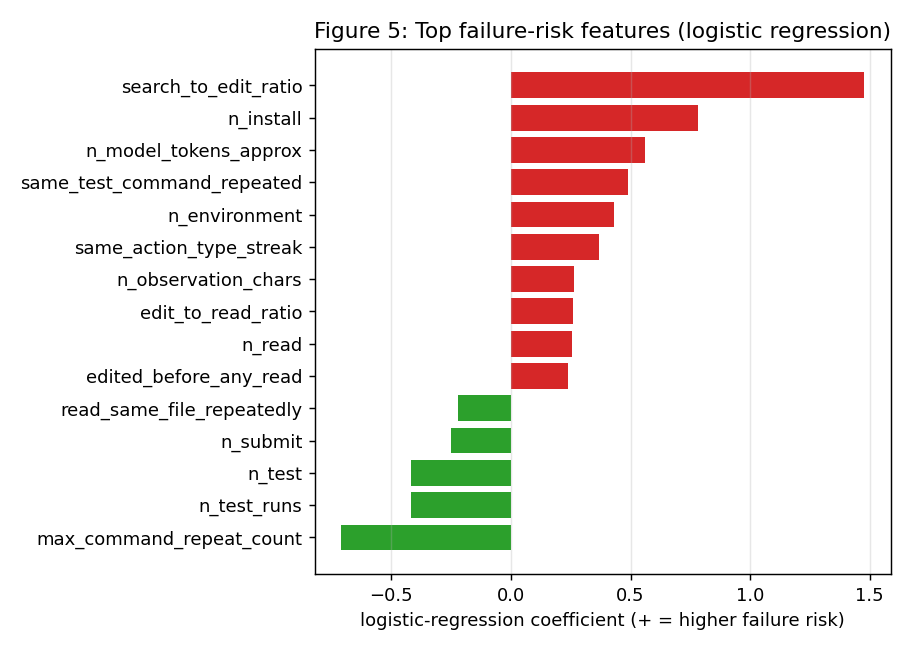
\includegraphics[width=.82\linewidth]{../results/figures/fig5_feature_importance_offline_full.png}
\caption{\textbf{Top failure-risk features} (logistic-regression coefficients). Repetition/looping signals and a high search-to-edit ratio raise risk; running tests and submitting lower it: ``visible flailing'' as the dominant signal.}
\end{figure}
\begin{figure}[t]\centering
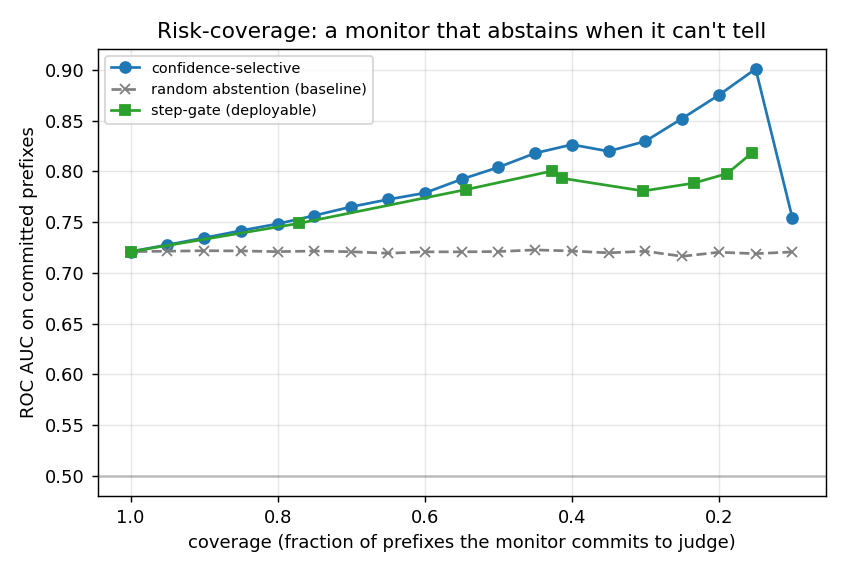
\includegraphics[width=.82\linewidth]{../results/figures/fig6_risk_coverage_offline_full.png}
\caption{\textbf{Risk-coverage (selective prediction).} Confidence-selective AUC rises to 0.80 @ 50\% coverage / 0.83 @ 30\%; a random-abstention control stays flat at 0.72 (the lift is real selection), and a deployable step-gate is shown for comparison.}
\end{figure}
\begin{figure}[t]\centering
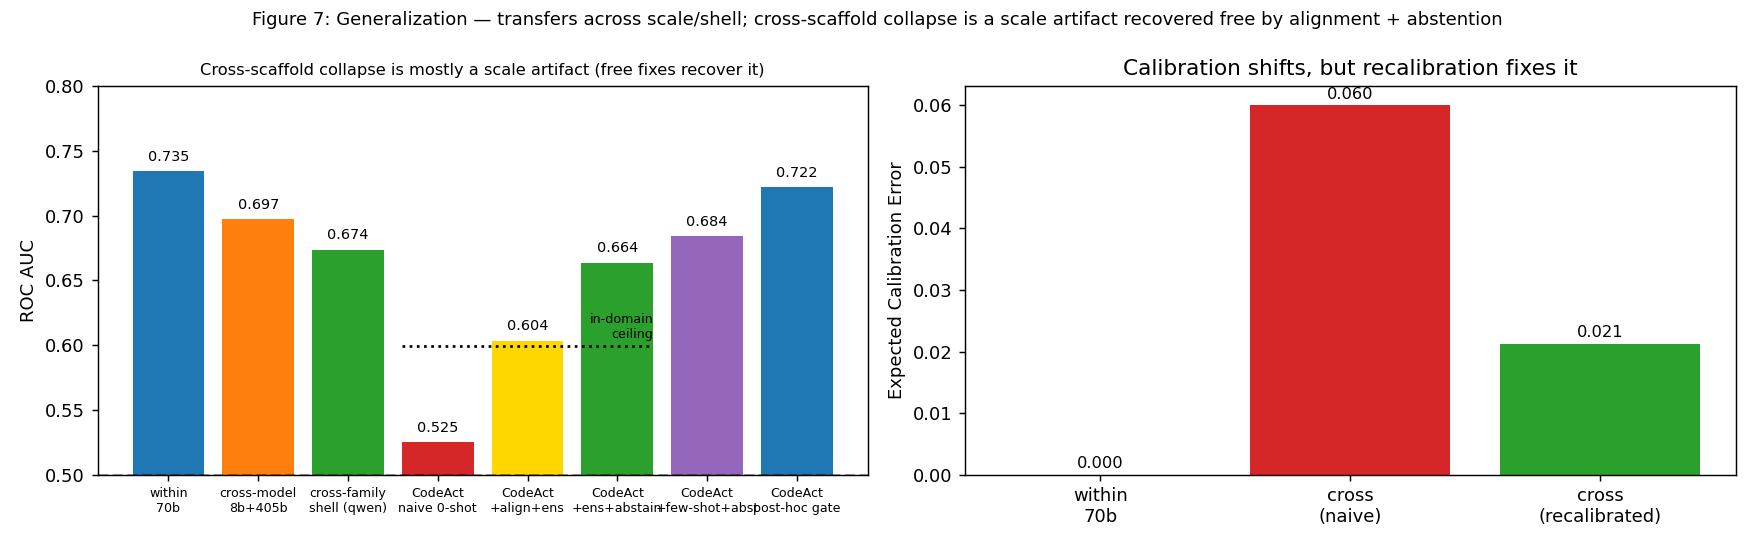
\includegraphics[width=.82\linewidth]{../results/figures/fig7_generalization.png}
\caption{\textbf{Generalization.} (left) Transfer AUC across model scale, a shell-style scaffold, and the cross-scaffold (CodeAct) collapse-then-free-recovery (naive 0.53 $\to$ +align+ensemble 0.60 $\to$ +abstention 0.66), with the in-domain ceiling marked; (right) calibration shifts cross- distribution but recalibration restores it (ECE 0.06$\to$0.02).}
\end{figure}
\begin{figure}[t]\centering
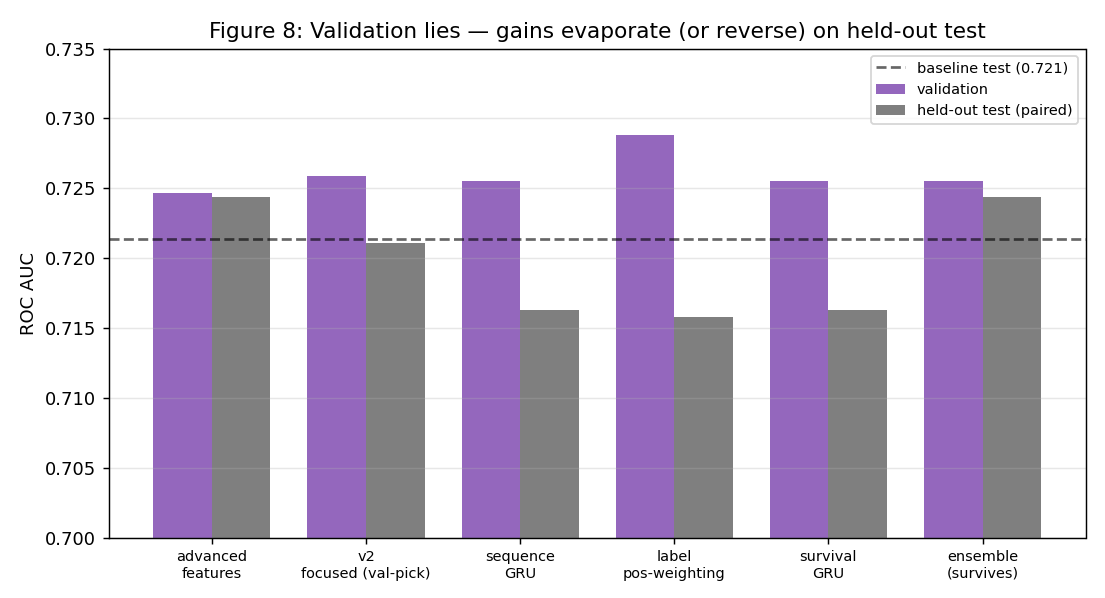
\includegraphics[width=.82\linewidth]{../results/figures/fig8_validation_lies.png}
\caption{\textbf{``Validation lies.''} Validation vs. paired instance-grouped held-out test AUC for five candidate improvements: each won on validation but was no better (or worse) on held-out test; only the ensemble survived, motivating the evaluation protocol (\S5).}
\end{figure}
\begin{figure}[t]\centering
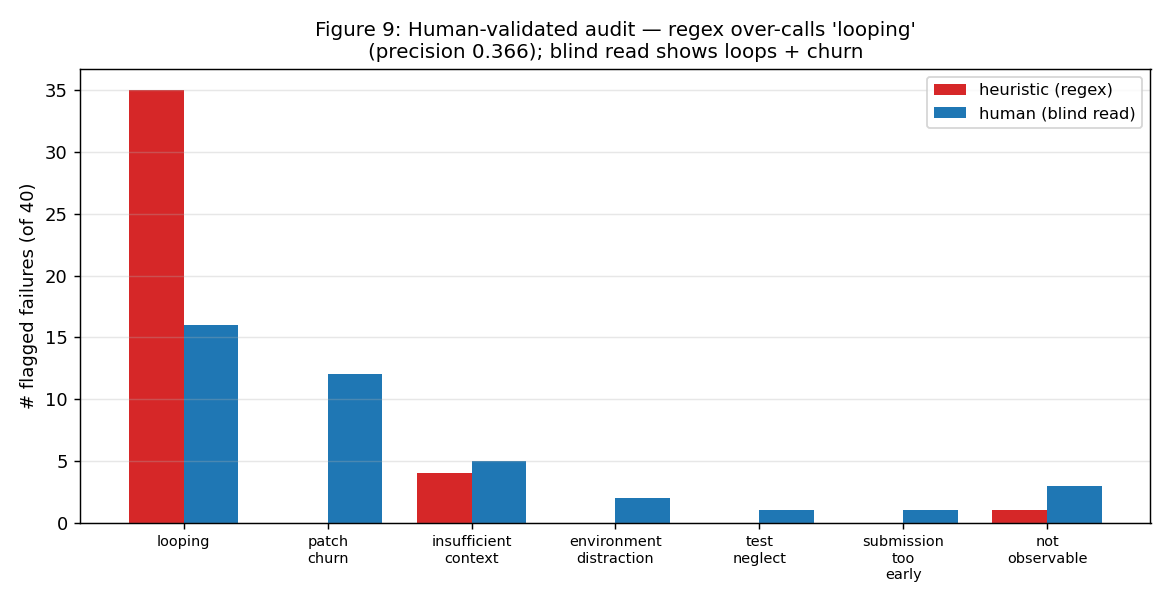
\includegraphics[width=.82\linewidth]{../results/figures/fig9_audit_validation.png}
\caption{\textbf{Human-validated failure-mode audit} (50 blind-labeled prefixes). The regex labeler over-calls ``looping'' (precision 0.37); blind human reading shows repetition + churn dominate the confidently-caught failures.}
\end{figure}
\begin{figure}[t]\centering
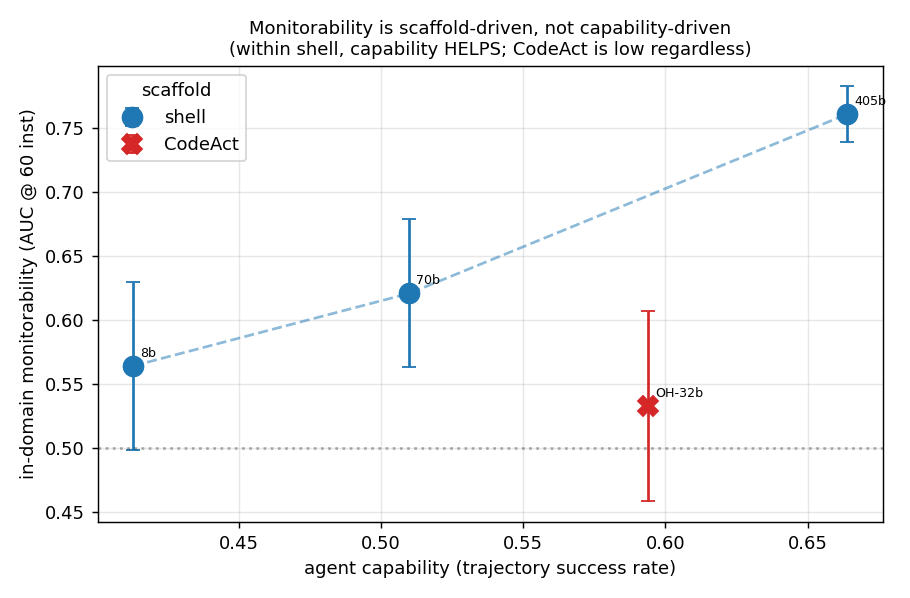
\includegraphics[width=.82\linewidth]{../results/figures/fig10_capability_monitorability.png}
\caption{\textbf{Monitorability vs. capability, at matched data budget.} Within the shell scaffold, monitorability \emph{rises} with capability (8b$\to$405b: 0.56$\to$0.76); the CodeAct agent is the \emph{least} monitorable despite mid-high capability: monitorability is scaffold-driven, not capability-driven.}
\end{figure}
\begin{figure}[t]\centering
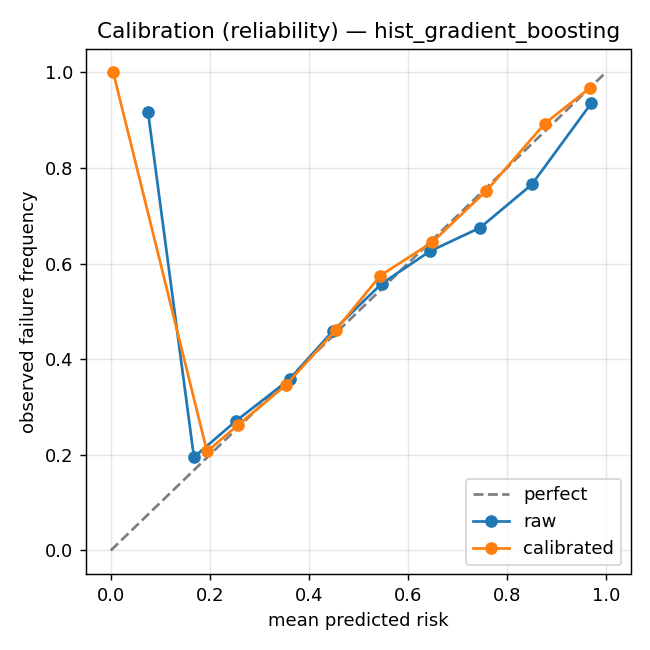
\includegraphics[width=.82\linewidth]{../results/figures/calibration_offline_full.png}
\caption{\textbf{Reliability diagram} for the deployed monitor, raw vs. isotonic-calibrated (ECE 0.011).}
\end{figure}
\section*{Reproducibility}
All figures/tables regenerate from saved artifacts via \texttt{python scripts/make\_report.py -{}-config configs/offline\_full.yaml} (no retraining). Key scripts: feature/label build and training under \texttt{scripts/}; generalization (\texttt{run\_generalization.py}) and the \textbf{second-source zero-shot test} (\texttt{ingest\_openhands.py} $\to$ \texttt{build\_prefix\_dataset.py} $\to$ \texttt{run\_second\_source.py}, reusing the same feature pipeline); abstention curves (\texttt{abstention.py}), online capture/replay (\texttt{run\_shadow\_capture.py}, \texttt{run\_monitor\_replay.py}), human audit (\texttt{build\_audit\_sample.py}, \texttt{score\_audit.py}), deployment cost (\texttt{measure\_cost.py}), and the LLM-judge baselines (\texttt{run\_openai\_judge\_subset.py -{}-backend \{openai,openrouter\}}, reusing one prompt/schema across \texttt{ollama\_judge.py}, \texttt{openai\_judge.py}, \texttt{openrouter\_judge.py}). Hardware: Apple M4 MacBook (10 cores, 32 GB RAM). \textbf{The monitor and all training/evaluation are local (Ollama, CPU, no GPU); the LLM-judge baseline alone uses paid APIs} (OpenAI, OpenRouter), pinned to dated model snapshots (\texttt{gpt-5.5-2026-04-23}, \texttt{claude-opus-4.8 -> claude-4.8-opus-20260528}) with per-call checkpointing. Test set scored once; all deltas reported with paired instance-bootstrap CIs.



\bibliography{refs}

\end{document}
